\chapter{AgentOS 的自指学习调度原理}

前面我们讨论了 AgentOS 的学习调度的基本运行机制，现在我们进一步深入探讨其自指学习调度的数学原理。

\section{问题定义：从参数学习到可塑性调度}

传统机器学习通常将学习写为参数优化：
\begin{equation}
\Theta_{k+1}
=
\Theta_k
-
\eta_k
\nabla_{\Theta}\mathcal{L}_k .
\end{equation}

对于持续运行的 Agent，该表示并不充分。原因在于：一次经验并不必然只应修改结构记忆
$\Theta$，而可能首先改变情景记忆 $E$，也可能改变记忆治理策略、认知控制策略、
资源调度策略、自我结构 $\Psi$ 或生命周期方向结构 $\Omega$。

因此，AgentOS 中的学习首先不是一个参数更新问题，而是一个结构修改分配问题。

设 Agent 在时刻 $t$ 的全部可塑结构集合为
\begin{equation}
\mathcal{X}_t
=
\{
E_t,
\Theta_t,
\Lambda_{E,t},
\Pi_{C,t},
\Pi_{S,t},
\Pi_{B,t},
\Psi_t,
\Omega_t
\},
\end{equation}
其中：

\begin{equation}
\Lambda_E
=
\text{情景记忆治理参数},
\end{equation}

\begin{equation}
\Pi_C
=
\text{认知控制与复杂度治理策略},
\end{equation}

\begin{equation}
\Pi_S
=
\text{资源与学习调度策略},
\end{equation}

\begin{equation}
\Pi_B
=
\text{边界与结构写入权限策略}.
\end{equation}

定义 AgentOS 学习为：
\begin{equation}
\boxed{
Learning
=
ExperienceDrivenChangeOfFutureStateTransition
}
\end{equation}

即：凡是经验驱动并能够持续改变未来状态转移规律的结构变化，都属于学习。

由此，AgentOS 学习问题可以重写为：
\begin{equation}
\boxed{
Experience
\rightarrow
CreditAssignment
\rightarrow
PlasticityAllocation
\rightarrow
StructureChange
}
\end{equation}

学习调度的核心任务因此变为：
\begin{equation}
\boxed{
\text{决定现实反馈应该获得改变 Agent 哪一部分结构的权力。}
}
\end{equation}

\begin{figure}[htbp]
\centering
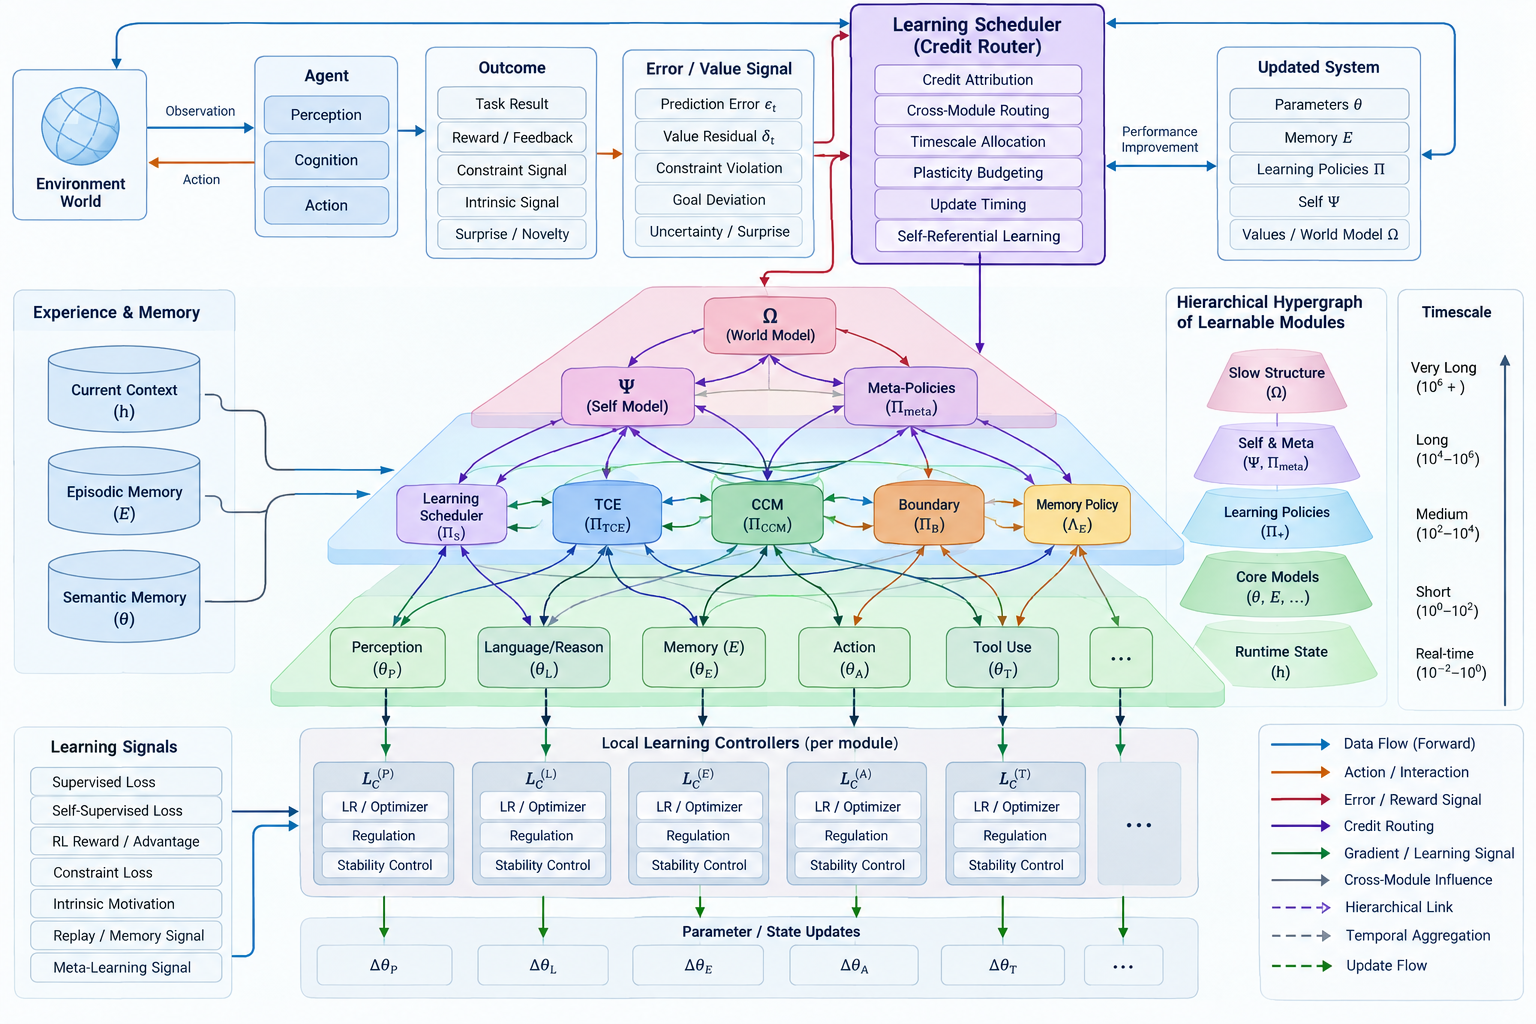
\includegraphics[width=.9\textwidth,height=.4\textheight,keepaspectratio]{images/struct.png}
\caption{自指递归调度器学习过程}
\end{figure}


\section{多尺度可塑性超图}

为了统一描述 AgentOS 中不同结构之间的学习依赖关系，定义多尺度可塑性超图：
\begin{equation}
\boxed{
\mathcal{H}_L
=
(
V_L,
\mathcal{E}_L,
W_L,
\mathcal{T}_L,
\mathcal{B}_L
)
}
\end{equation}

其中：

\begin{equation}
V_L
=
\{v_1,v_2,\ldots,v_n\}
\end{equation}
表示全部可塑结构节点；

\begin{equation}
\mathcal{E}_L
\end{equation}
表示结构之间的学习依赖超边；

\begin{equation}
W_L
\end{equation}
表示信用传播权重；

\begin{equation}
\mathcal{T}_L
=
\{\tau_1,\tau_2,\ldots,\tau_n\}
\end{equation}
表示各节点的特征学习时间尺度；

\begin{equation}
\mathcal{B}_L
=
\{B_1^P,B_2^P,\ldots,B_n^P\}
\end{equation}
表示各节点的可塑性预算。

典型节点包括：
\begin{equation}
V_L
\supset
\{
E,
\Theta,
\Lambda_E,
\Pi_C,
\Pi_S,
\Pi_B,
\Psi,
\Omega
\}.
\end{equation}

由于一个结果通常由多个结构共同产生，因此一般有：
\begin{equation}
\mathcal{H}_L
\neq
\text{Tree}.
\end{equation}

更准确地说：
\begin{equation}
\boxed{
\mathcal{H}_L
=
\text{Hierarchical Multi-timescale Plasticity Hypergraph}
}
\end{equation}

其几何直觉为多层金字塔，但其拓扑结构允许：

\begin{equation}
\text{one-to-many},
\qquad
\text{many-to-one},
\qquad
\text{cross-level coupling}.
\end{equation}


\section{学习信号空间}

定义时刻 $t$ 的学习信号向量：
\begin{equation}
\mathbf{s}_t^L
=
\left[
s_t^{sup},
s_t^{pred},
s_t^{rew},
s_t^{sur},
s_t^{nov},
s_t^{con},
s_t^{cost},
s_t^{cons}
\right].
\end{equation}

其中：

\begin{equation}
s_t^{sup}
=
\text{监督信号},
\end{equation}

\begin{equation}
s_t^{pred}
=
\varepsilon_t
=
D(\hat h_{t+1},h_{t+1}),
\end{equation}

\begin{equation}
s_t^{rew}
=
r_t,
\end{equation}

\begin{equation}
s_t^{sur}
=
\text{惊奇信号},
\end{equation}

\begin{equation}
s_t^{nov}
=
\text{新颖性信号},
\end{equation}

\begin{equation}
s_t^{con}
=
\text{约束违反信号},
\end{equation}

\begin{equation}
s_t^{cost}
=
\text{资源成本信号},
\end{equation}

\begin{equation}
s_t^{cons}
=
\text{跨时间一致性信号}.
\end{equation}

重要的是：
\begin{equation}
\boxed{
LearningSignal
\neq
LearningTarget
}
\end{equation}

同一个误差信号可以被分配给不同结构，而同一个结构也可以同时接收多种学习信号。


\section{信用作为学习调度的基本变量}

定义节点 $v_i$ 在时刻 $t$ 获得的信用为：
\begin{equation}
c_i(t).
\end{equation}

信用并不一定表示正奖励，也可表示责任、误差归因或结构修改需求。

定义全局信用向量：
\begin{equation}
\mathbf{c}_t
=
[
c_1(t),
c_2(t),
\ldots,
c_n(t)
].
\end{equation}

学习调度器的基本映射为：
\begin{equation}
\boxed{
\mathcal{R}_L:
(\mathbf{s}_t^L,\mathcal{X}_t,\mathcal{H}_L)
\rightarrow
\mathbf{c}_t
}
\end{equation}

因此学习调度的本体可以定义为：
\begin{equation}
\boxed{
LearningScheduling
=
CreditRoutingOnPlasticityHypergraph
}
\end{equation}

若采用归一化信用表示，则可以令：
\begin{equation}
c_i(t)\geq 0,
\end{equation}

\begin{equation}
\sum_i c_i(t)=1.
\end{equation}

若希望同时表达学习强度，则无需归一化，而采用：
\begin{equation}
\sum_i |c_i(t)|
\leq
B_L(t),
\end{equation}
其中 $B_L(t)$ 为当前总学习信用预算。


\section{信用不是标量，而是多通道向量}

由于 AgentOS 同时存在监督、自监督、强化、约束与资源反馈，因此更一般地定义节点信用：
\begin{equation}
\mathbf{c}_i(t)
=
\left[
c_i^{sup},
c_i^{self},
c_i^{RL},
c_i^{constraint},
c_i^{cost}
\right].
\end{equation}

于是同一结构可以同时接收不同来源的学习压力：
\begin{equation}
\mathbf{c}_i
\in
\mathbb{R}^{d_c}.
\end{equation}

局部更新不再简单写为：
\begin{equation}
\Delta\xi_i
\propto
c_i,
\end{equation}
而应写为：
\begin{equation}
\boxed{
\Delta\xi_i
=
\mathcal{A}_i
(
\xi_i,
\mathbf{c}_i,
\mathbf{u}_i^L
)
}
\end{equation}

其中 $\mathbf{u}_i^L$ 是 Learning Control 输出的局部学习控制变量。


\section{三层学习结构}

AgentOS 的全部学习过程可以压缩为三个功能层级：
\begin{equation}
\boxed{
LearningScheduling
\rightarrow
LearningControl
\rightarrow
LearningAdaptation
}
\end{equation}

三层分别对应：
\begin{equation}
\boxed{
CreditRouting
\rightarrow
CreditTransformation
\rightarrow
CreditRealization
}
\end{equation}


\section{第一层：学习调度}

学习调度解决：
\begin{equation}
\boxed{
\text{谁获得学习信用？}
}
\end{equation}

定义调度器：
\begin{equation}
\mathbf{g}_t
=
S_{\Phi_S}
(
\mathcal{X}_t,
\mathbf{s}_t^L,
B_L(t)
),
\end{equation}
其中：
\begin{equation}
\mathbf{g}_t
=
[g_1,g_2,\ldots,g_n],
\qquad
g_i\in[0,1].
\end{equation}

$g_i$ 表示节点 $v_i$ 获得结构修改资格的程度。

信用最终可以写为：
\begin{equation}
\mathbf{c}_i
=
g_i
\,
\mathcal{Q}_i(
\mathbf{s}_t^L,
\mathcal{X}_t
).
\end{equation}

因此：
\begin{equation}
g_i\approx0
\end{equation}
意味着即使存在误差，该结构当前仍然不获得学习权限。


\section{第二层：学习控制}

Learning Control 解决：
\begin{equation}
\boxed{
\text{获得信用以后应该怎样学习？}
}
\end{equation}

定义：
\begin{equation}
\mathbf{u}_i^L
=
C_{\Phi_C}
(
\xi_i,
\mathbf{c}_i,
\mathcal{X}_t
).
\end{equation}

其中：
\begin{equation}
\mathbf{u}_i^L
=
[
\eta_i,
B_i^P,
M_i,
K_i,
R_i,
\alpha_i^{sup},
\alpha_i^{self},
\alpha_i^{RL},
\ldots
].
\end{equation}

分别可以控制：

\begin{equation}
\eta_i
=
\text{有效学习率},
\end{equation}

\begin{equation}
B_i^P
=
\text{局部可塑性预算},
\end{equation}

\begin{equation}
M_i
=
\text{允许修改的结构掩码},
\end{equation}

\begin{equation}
K_i
=
\text{更新步数},
\end{equation}

\begin{equation}
R_i
=
\text{Replay 强度},
\end{equation}

以及不同学习算子的组合权重。


\section{第三层：学习适应}

Learning Adaptation 执行真正的结构变化：
\begin{equation}
\boxed{
\xi_i(t+1)
=
\xi_i(t)
+
\Delta\xi_i(t)
}
\end{equation}

其中：
\begin{equation}
\Delta\xi_i
=
\sum_k
\alpha_{ik}
\mathcal{A}_{ik}
(
\xi_i,\mathbf{s}_t^L
).
\end{equation}

这里 $\mathcal{A}_{ik}$ 可以是：

\begin{equation}
\mathcal{A}^{sup}
\end{equation}
监督更新；

\begin{equation}
\mathcal{A}^{self}
\end{equation}
自监督更新；

\begin{equation}
\mathcal{A}^{RL}
\end{equation}
强化学习更新；

\begin{equation}
\mathcal{A}^{replay}
\end{equation}
重放更新；

\begin{equation}
\mathcal{A}^{local}
\end{equation}
局部可塑性更新；

\begin{equation}
\mathcal{A}^{struct}
\end{equation}
结构重组更新。

因此：
\begin{equation}
\boxed{
SupervisedLearning,
SelfSupervisedLearning,
ReinforcementLearning
}
\end{equation}

在 AgentOS 中不再是顶层学习结构，而是：
\begin{equation}
\boxed{
LearningAdaptationOperators.
}
\end{equation}


\section{三相记忆是最基本的信用沉降路径}

对于三相记忆：
\begin{equation}
h
\rightarrow
E
\rightarrow
\Theta,
\end{equation}
可以重新解释为：
\begin{equation}
\boxed{
InstantError
\rightarrow
EpisodeCredit
\rightarrow
StructuralCredit.
}
\end{equation}

当前预测残差：
\begin{equation}
\varepsilon_t
=
D(
\hat h_{t+1},
h_{t+1}
)
\end{equation}
首先不应默认直接全部作用于 $\Theta$。

对于单次异常，可令：
\begin{equation}
c_E\gg0,
\end{equation}

\begin{equation}
c_\Theta\approx0.
\end{equation}

经过多个 Episode：
\begin{equation}
E_1,E_2,\ldots,E_n
\end{equation}
后，如果某种残差结构持续存在，则结构信用逐渐积累：
\begin{equation}
c_\Theta
=
F(
Support,
Confidence,
Coverage,
ResidualPersistence
).
\end{equation}

于是：
\begin{equation}
\boxed{
h
\rightarrow
E
\rightarrow
\Theta
}
\end{equation}
不仅是记忆相变，也是一条信用从快速状态向慢结构沉降的基本路径。


\section{结构信用的时间积累}

定义某一结构模式 $\rho$ 的累计信用：
\begin{equation}
C_\rho(t)
=
\int_{0}^{t}
K_\rho(t-\tau)
\,
\varepsilon_\rho(\tau)
\,d\tau .
\end{equation}

其中：
\begin{equation}
K_\rho(\Delta t)
\end{equation}
为时间信用核。

若采用指数核：
\begin{equation}
K_\rho(\Delta t)
=
\exp
\left(
-\frac{\Delta t}{\tau_\rho}
\right),
\end{equation}
则：
\begin{equation}
\tau_\rho
\end{equation}
决定一个结构需要多长的历史支持才能获得显著信用。

对于不同层级：
\begin{equation}
\tau_E
<
\tau_\Theta
<
\tau_\Psi
<
\tau_\Omega
\end{equation}
可以作为一种默认稳定性设计关系，而不是自然定律。


\section{Eligibility Trace 与延迟信用}

现实反馈经常晚于导致结果的学习决策。

定义节点 $i$ 的学习资格痕迹：
\begin{equation}
e_i^L(t)
=
\gamma_e
e_i^L(t-1)
+
\phi_i(t),
\end{equation}
其中：
\begin{equation}
0\leq\gamma_e<1.
\end{equation}

当延迟结果 $r_t$ 到达时：
\begin{equation}
c_i(t)
=
e_i^L(t)
\delta_t,
\end{equation}
其中 $\delta_t$ 为当前价值残差或长期结果误差。

因此：
\begin{equation}
\boxed{
EligibilityTrace
=
TemporalBridgeForDelayedCredit
}
\end{equation}

它允许过去的：

\begin{equation}
\text{记忆写入决策},
\end{equation}

\begin{equation}
\text{Theta 更新决策},
\end{equation}

\begin{equation}
\text{调度决策}
\end{equation}

接受未来结果的责任归因。


\section{信用在超图中的传播}

对于普通图，可以定义：
\begin{equation}
c_j^{(l+1)}
=
\sum_i
g_{i\rightarrow j}
c_i^{(l)}.
\end{equation}

其中：
\begin{equation}
g_{i\rightarrow j}
\in[0,1]
\end{equation}
为信用传播门。

在超图中，一条超边：
\begin{equation}
e
=
\{v_{i_1},v_{i_2},\ldots,v_{i_k}\}
\end{equation}
允许多个结构共同对同一结果负责。

因此更一般地：
\begin{equation}
\boxed{
c_v^{(l+1)}
=
\sum_{e\ni v}
\alpha_{e,v}
\,
\Phi_e
\left(
\{c_u^{(l)}:u\in e\},
\mathcal{X}_t
\right)
}
\end{equation}

其中：
\begin{equation}
\Phi_e
\end{equation}
是该超边的联合信用函数。

这允许表示：
\begin{equation}
\text{Knowledge}
+
\text{MemoryPolicy}
+
\text{ControlPolicy}
\rightarrow
\text{JointOutcome}.
\end{equation}


\section{纵向、横向与跨时间尺度信用}

AgentOS 中至少存在三类信用传播。

纵向传播：
\begin{equation}
Outcome
\rightarrow
Policy
\rightarrow
Parameter.
\end{equation}

横向传播：
\begin{equation}
\Theta
\leftrightarrow
E
\leftrightarrow
\Pi_C
\leftrightarrow
\Pi_S.
\end{equation}

跨时间尺度传播：
\begin{equation}
\boxed{
InstantResidual
\rightarrow
EpisodeCredit
\rightarrow
StructuralCredit
\rightarrow
SelfCredit.
}
\end{equation}

因此 Learning Scheduler 不是一个单层分类器，而是一个：
\begin{equation}
\boxed{
Multi-scale Credit Routing Process.
}
\end{equation}


\section{学习权限与可塑性预算}

定义节点 $i$ 的可塑性预算：
\begin{equation}
B_i^P(t)\geq0.
\end{equation}

学习更新必须满足：
\begin{equation}
\boxed{
\|\Delta\xi_i\|
\leq
B_i^P(t).
}
\end{equation}

全局还满足：
\begin{equation}
\boxed{
\sum_i
C_i^{learn}(t)
\leq
B_L(t).
}
\end{equation}

因此：
\begin{equation}
\boxed{
Plasticity
=
FiniteAgentResource.
}
\end{equation}

对于快慢结构，可以采用默认关系：
\begin{equation}
B_E^P
>
B_\Theta^P
>
B_\Psi^P.
\end{equation}

该关系表达的是稳定性设计原则：

\begin{equation}
\boxed{
\text{结构越慢，单位时间允许的修改幅度越小。}
}
\end{equation}


\section{慢结构保护原则}

定义结构 $i$ 的稳定尺度：
\begin{equation}
\tau_i.
\end{equation}

则允许的平均可塑性强度可设计为：
\begin{equation}
\bar B_i^P
\propto
\frac{1}{\tau_i}.
\end{equation}

更一般地：
\begin{equation}
B_i^P
=
F_B(
\tau_i,
Confidence_i,
Risk_i,
Support_i
).
\end{equation}

从而：
\begin{equation}
\boxed{
SlowStructure
\Rightarrow
HighEvidenceThreshold
+
LowPlasticityRate.
}
\end{equation}


\section{E 到 Theta 的信用升级}

对情景记忆 $E_i$，定义其结构学习资格：
\begin{equation}
Q_i^\Theta
=
\sigma
\left(
w_s S_i
+
w_c C_i
+
w_v V_i
+
w_r R_i
+
w_u U_i
-
w_f F_i
\right).
\end{equation}

其中：

\begin{equation}
S_i
=
Support_i,
\end{equation}

\begin{equation}
C_i
=
Confidence_i,
\end{equation}

\begin{equation}
V_i
=
Coverage_i,
\end{equation}

\begin{equation}
R_i
=
ResidualPersistence_i,
\end{equation}

\begin{equation}
U_i
=
FutureUtility_i,
\end{equation}

\begin{equation}
F_i
=
Conflict_i.
\end{equation}

结构写入信用为：
\begin{equation}
c_\Theta^{(i)}
=
g_\Theta
Q_i^\Theta.
\end{equation}

于是：
\begin{equation}
\boxed{
Episode
\rightarrow
EvidenceAccumulation
\rightarrow
StructuralCredit.
}
\end{equation}


\section{Theta 对 E 的间接反向作用}

结构记忆更新：
\begin{equation}
\Theta_t
\rightarrow
\Theta_{t+1}
\end{equation}
会改变未来工作状态生成：
\begin{equation}
\hat h_{t+1}
=
F_{\Theta_{t+1}}(h_t,u_t).
\end{equation}

如果结构学习成功，则：
\begin{equation}
\varepsilon_{t+1}\downarrow.
\end{equation}

进一步导致：
\begin{equation}
Recall(E_i)\downarrow,
\end{equation}

\begin{equation}
Reinforcement(E_i)\downarrow,
\end{equation}

最终：
\begin{equation}
m_i(E)\downarrow.
\end{equation}

因此：
\begin{equation}
\boxed{
\Theta
\rightarrow
BetterPrediction
\rightarrow
LessSurprise
\rightarrow
LessRecall
\rightarrow
EpisodeEvaporation
}
\end{equation}

比直接：
\begin{equation}
\Theta\rightarrow Delete(E)
\end{equation}
更符合三相记忆的连续动力学。


\section{E 治理策略也是可塑节点}

定义情景记忆治理参数：
\begin{equation}
\Lambda_E
=
\{
\lambda_{evap},
\theta_{write},
\theta_{recall},
\beta_{surprise},
\tau_{cons},
\ldots
\}.
\end{equation}

这些变量决定：
\begin{equation}
WhatToRemember,
\end{equation}

\begin{equation}
WhatToRecall,
\end{equation}

\begin{equation}
WhatToForget,
\end{equation}

\begin{equation}
WhatToConsolidate.
\end{equation}

因此：
\begin{equation}
\boxed{
\Lambda_E
=
MemoryGovernancePolicy.
}
\end{equation}

定义长期记忆治理效用：
\begin{equation}
J_E
=
U_{future}
-
\alpha C_{storage}
-
\beta C_{recall}
-
\gamma C_{false}
-
\delta C_{update}.
\end{equation}

则：
\begin{equation}
\Lambda_{E,t+1}
=
\Lambda_{E,t}
+
\eta_E
\widehat{\nabla}_{\Lambda_E}
J_E.
\end{equation}

这构成：
\begin{equation}
\boxed{
LearningToRemember.
}
\end{equation}


\section{Psi 的信用升级条件}

自我结构 $\Psi$ 不应响应单次异常事件。

定义 Episode $E_i$ 对 $\Psi$ 的更新资格：
\begin{equation}
Q_i^\Psi
=
f(
SelfRelevance_i,
Persistence_i,
CrossContextSupport_i,
Confidence_i
).
\end{equation}

只有当：
\begin{equation}
Q_i^\Psi
>
\theta_\Psi
\end{equation}
时，才允许：
\begin{equation}
c_\Psi>0.
\end{equation}

因此：
\begin{equation}
\boxed{
EpisodeCredit
\not\Rightarrow
SelfCredit.
}
\end{equation}

只有跨时间、跨情景、持续稳定的自我相关证据，才能获得慢自我结构的修改权限。


\section{Omega 的超慢信用积累}

生命周期方向结构 $\Omega$ 的更新资格应依赖更长时间尺度：

\begin{equation}
Q^\Omega
=
f(
LongTermOutcome,
GoalConsistency,
RepeatedTrajectory,
\Psi
).
\end{equation}

因此通常有：
\begin{equation}
\tau_\Omega
>
\tau_\Psi.
\end{equation}

并且：
\begin{equation}
B_\Omega^P
<
B_\Psi^P.
\end{equation}

这保证生命周期方向不会被短期局部奖励轻易改写。


\section{Boundary 对学习权限的治理}

外部信息进入工作状态并不等于拥有长期结构写入权限。

定义三级权限：
\begin{equation}
P_{observe},
\qquad
P_{remember},
\qquad
P_{consolidate}.
\end{equation}

一般设计为：
\begin{equation}
\boxed{
P_{observe}
\geq
P_{remember}
\geq
P_{consolidate}.
}
\end{equation}

因此：
\begin{equation}
Input
\rightarrow
h
\end{equation}
并不自动意味着：
\begin{equation}
Input
\rightarrow
\Theta.
\end{equation}

未经验证的信息可以：
\begin{equation}
h\rightarrow E,
\end{equation}
但：
\begin{equation}
E\nrightarrow\Theta
\end{equation}
直到结构信用达到要求。


\section{CCM 对学习调度的约束}

学习本身消耗工作记忆、计算与时间资源。

设当前认知负载：
\begin{equation}
L_C(t).
\end{equation}

当：
\begin{equation}
L_C(t)
\rightarrow
L_{critical},
\end{equation}
则应降低高成本学习活动：
\begin{equation}
g_\Theta\downarrow,
\end{equation}

同时仍可允许：
\begin{equation}
g_E>0.
\end{equation}

因此：
\begin{equation}
\boxed{
HighLoad
\Rightarrow
RecordNow,
ConsolidateLater.
}
\end{equation}

由此形成：
\begin{equation}
OnlineExperiencePhase
\end{equation}
与：
\begin{equation}
OfflineConsolidationPhase
\end{equation}
的时间分离。


\section{Scheduler 与 Learning Scheduler 的关系}

普通 Scheduler 分配：
\begin{equation}
Compute,
Memory,
Tool,
Time.
\end{equation}

Learning Scheduler 分配：
\begin{equation}
Plasticity,
LearningCredit,
StructuralWritePermission.
\end{equation}

因此 AgentOS Scheduler 可以统一写为：
\begin{equation}
\boxed{
Scheduler
=
ResourceScheduling
+
ProcessScheduling
+
LearningScheduling.
}
\end{equation}

其中 Learning Scheduling 的特殊资源为：
\begin{equation}
\boxed{
PlasticityBudget.
}
\end{equation}


\section{学习冲突}

一个节点可能同时获得多个方向不一致的学习信号。

若：
\begin{equation}
\mathbf{g}_a
\cdot
\mathbf{g}_b
<
0,
\end{equation}
则发生梯度冲突。

更一般地，AgentOS 学习冲突包括：

\begin{equation}
GradientConflict,
\end{equation}

\begin{equation}
TimescaleConflict,
\end{equation}

\begin{equation}
GoalConflict,
\end{equation}

\begin{equation}
StructuralStabilityConflict.
\end{equation}

Learning Control 应求解受约束优化：
\begin{equation}
\min_{\Delta\xi}
\mathcal{L}_{task}(\xi+\Delta\xi)
\end{equation}
subject to
\begin{equation}
\|\Delta\xi\|
\leq
B_i^P,
\end{equation}

\begin{equation}
C_{risk}(\Delta\xi)
\leq
R_{\max},
\end{equation}

\begin{equation}
C_{stability}(\Delta\xi)
\leq
S_{\max}.
\end{equation}

因此：
\begin{equation}
\boxed{
Learning
=
ConstrainedStructuralControl.
}
\end{equation}


\section{学习调度器的自指条件}

令 Learning Scheduler 的参数为：
\begin{equation}
\Phi_S.
\end{equation}

因为：
\begin{equation}
\Phi_S
\in
V_L,
\end{equation}
所以调度器本身也是可塑性超图节点。

因此：
\begin{equation}
\boxed{
CreditRouter
\in
CreditGraph.
}
\end{equation}

它对其他结构分配信用，同时自身也可能因长期调度结果获得信用。

设调度器产生：
\begin{equation}
g_t
=
S_{\Phi_S}(X_t,s_t).
\end{equation}

其调度行为最终产生长期结果：
\begin{equation}
J_{t:T}.
\end{equation}

则调度器本身获得：
\begin{equation}
c_{\Phi_S}
=
\widehat{
\frac{\partial J_{t:T}}
{\partial \Phi_S}
}.
\end{equation}

并更新：
\begin{equation}
\boxed{
\Phi_{S,t+1}
=
\Phi_{S,t}
+
\eta_S
c_{\Phi_S}.
}
\end{equation}

这就是 AgentOS 学习调度的自指闭环。


\section{自指不是无限元递归}

自指学习不定义为：
\begin{equation}
S_1
\rightarrow
S_2
\rightarrow
S_3
\rightarrow
\cdots.
\end{equation}

而定义为：
\begin{equation}
\boxed{
S_t
\rightarrow
Outcome_t
\rightarrow
S_{t+1}.
}
\end{equation}

因此它是动力学递归：
\begin{equation}
x_{t+1}=F(x_t),
\end{equation}
而不是无限结构递归。

由此可定义：
\begin{equation}
\boxed{
MetaLearningDepth<\infty.
}
\end{equation}


\section{Learning Controller 的自适应}

Learning Controller 参数：
\begin{equation}
\Phi_C
\end{equation}
同样属于：
\begin{equation}
V_L.
\end{equation}

其输出：
\begin{equation}
u_t^L
=
C_{\Phi_C}(X_t,c_t)
\end{equation}
决定：

\begin{equation}
LearningRate,
\end{equation}

\begin{equation}
Replay,
\end{equation}

\begin{equation}
UpdateMask,
\end{equation}

\begin{equation}
GradientCombination,
\end{equation}

\begin{equation}
PlasticityBudget.
\end{equation}

若过去控制策略导致：

\begin{equation}
LearningInstability\uparrow
\end{equation}
或：
\begin{equation}
LearningEfficiency\downarrow,
\end{equation}
则：
\begin{equation}
\Phi_C
\rightarrow
\Phi_C'.
\end{equation}

因此：
\begin{equation}
\boxed{
LearningControl
}
\end{equation}
也属于自适应对象。


\section{调度器的长期目标}

Learning Scheduler 不应优化瞬时损失下降，而应优化长期综合效用。

定义：
\begin{equation}
\boxed{
J_S
=
J_{task}
-
\lambda_1 C_{learn}
-
\lambda_2 C_{forget}
-
\lambda_3 C_{instability}
-
\lambda_4 C_{memory}
-
\lambda_5 C_{risk}.
}
\end{equation}

其中：

\begin{equation}
C_{learn}
=
\text{学习计算成本},
\end{equation}

\begin{equation}
C_{forget}
=
\text{旧结构破坏成本},
\end{equation}

\begin{equation}
C_{instability}
=
\text{系统漂移成本},
\end{equation}

\begin{equation}
C_{memory}
=
\text{情景历史维护成本},
\end{equation}

\begin{equation}
C_{risk}
=
\text{错误慢结构更新风险}.
\end{equation}

因此：
\begin{equation}
\boxed{
LearningScheduler
\neq
FastLossMinimizer.
}
\end{equation}

更准确是：
\begin{equation}
\boxed{
LearningScheduler
=
LongHorizonPlasticityPolicy.
}
\end{equation}


\section{学习调度可以表述为强化控制问题}

定义 Learning Action：
\begin{equation}
a_t^L
=
(
g_t,
u_t^L
).
\end{equation}

状态：
\begin{equation}
s_t^A
=
(
X_t,
s_t^L,
B_L,
L_C
).
\end{equation}

则学习调度可以写成：
\begin{equation}
a_t^L
\sim
\pi_L(
a^L|s_t^A
).
\end{equation}

长期目标：
\begin{equation}
\boxed{
\max_{\pi_L}
\mathbb{E}
\left[
\sum_{t=0}^{\infty}
\gamma^t
r_t^L
\right]
}
\end{equation}

其中：
\begin{equation}
r_t^L
=
R_t^{task}
-
C_t^{learning}
-
C_t^{forgetting}
-
C_t^{instability}.
\end{equation}

因此学习调度可以采用强化学习技术，但强化学习只是其一种可能实现。


\section{调度器的反事实信用}

仅根据真实执行路径可能难以判断：
\begin{equation}
\text{“如果当时把信用分给另一个结构会怎样？”}
\end{equation}

定义反事实结果：
\begin{equation}
J^{cf}
(
a_t^{L'}
).
\end{equation}

则调度动作优势：
\begin{equation}
A_L(
s_t,
a_t^L
)
=
J(
a_t^L
)
-
\mathbb{E}_{a_t^{L'}}
[
J^{cf}(a_t^{L'})
].
\end{equation}

于是调度器可以利用：
\begin{equation}
\boxed{
CounterfactualCreditAssignment
}
\end{equation}
估计某次结构信用分配是否合理。


\section{自指学习的稳定性约束}

设整个学习系统：
\begin{equation}
X_{t+1}
=
F_L(
X_t,s_t
).
\end{equation}

局部稳定性可以通过 Jacobian：
\begin{equation}
J_L
=
\frac{\partial F_L}
{\partial X}
\end{equation}
分析。

在线性化邻域内，一个充分但非必要的局部收敛条件为：
\begin{equation}
\boxed{
\rho(J_L)<1,
}
\end{equation}
其中 $\rho$ 为谱半径。

这不是 AgentOS 必须全局满足的物理定律，而是用于表达一个重要设计原则：

\begin{equation}
\boxed{
\text{学习闭环本身必须保持有界。}
}
\end{equation}


\section{自指学习的慢变量保护}

为了避免：
\begin{equation}
BadScheduler
\rightarrow
BadLearning
\rightarrow
WorseScheduler,
\end{equation}
需要限制自修改强度。

可采用：
\begin{equation}
\|\Delta\Phi_S\|
\leq
B_S,
\end{equation}

\begin{equation}
\eta_S
\ll
\eta_{local},
\end{equation}

以及：
\begin{equation}
J_S^{new}
>
J_S^{old}
-
\epsilon
\end{equation}
等保守接受条件。

因此：
\begin{equation}
\boxed{
SelfReference
\neq
UnboundedSelfModification.
}
\end{equation}

而应满足：
\begin{equation}
\boxed{
SelfReferentialLearning
=
BoundedRecursiveAdaptation.
}
\end{equation}


\section{连续学习动力学与离散学习治理}

AgentOS 中并非所有学习过程都必须可微。

连续部分可写为：
\begin{equation}
\dot\xi_i
=
F_i(
\xi_i,c_i,u_i^L
).
\end{equation}

而离散治理可以包括：
\begin{equation}
Merge,
\end{equation}

\begin{equation}
Split,
\end{equation}

\begin{equation}
Freeze,
\end{equation}

\begin{equation}
Activate,
\end{equation}

\begin{equation}
Consolidate,
\end{equation}

\begin{equation}
Offload.
\end{equation}

因此整体学习系统更适合写成混合动力系统：
\begin{equation}
\boxed{
\mathcal{L}_{Agent}
=
ContinuousPlasticity
\bowtie
DiscreteLearningGovernance.
}
\end{equation}


\section{多时间尺度学习方程}

设第 $i$ 个结构具有：
\begin{equation}
\tau_i.
\end{equation}

则可以统一写成：
\begin{equation}
\boxed{
\tau_i
\dot\xi_i
=
g_i(t)
F_i(
\xi_i,
\mathbf{c}_i,
\mathbf{u}_i^L
).
}
\end{equation}

其中：

\begin{equation}
g_i(t)
\end{equation}
决定是否获得学习权限；

\begin{equation}
\mathbf{c}_i
\end{equation}
决定为什么改变；

\begin{equation}
\mathbf{u}_i^L
\end{equation}
决定怎样改变；

\begin{equation}
\tau_i
\end{equation}
决定改变速度。

这给出 AgentOS 学习调度的一个核心统一微分形式。


\section{信用扩散的连续近似}

如果将大量可塑结构视为连续结构空间 $\mathcal{M}_L$，可定义信用场：
\begin{equation}
c(x,t).
\end{equation}

其演化可抽象为：
\begin{equation}
\boxed{
\frac{\partial c}{\partial t}
=
-\nabla\cdot
(
v_c c
)
+
\nabla\cdot
(
D_c\nabla c
)
+
S_c
-
\Gamma_c c.
}
\end{equation}

其中：

\begin{equation}
v_c
=
\text{信用定向迁移场},
\end{equation}

\begin{equation}
D_c
=
\text{信用扩散张量},
\end{equation}

\begin{equation}
S_c
=
\text{新误差、奖励与约束产生的信用源},
\end{equation}

\begin{equation}
\Gamma_c
=
\text{信用衰减与抑制}.
\end{equation}

该方程不是对 AgentOS 必须采用连续 PDE 实现的要求，而是对多尺度信用传播的连续极限表示。


\section{金字塔中的信用上迁}

设结构层级为：
\begin{equation}
L_0,L_1,\ldots,L_K.
\end{equation}

底层代表快速、具体结构，上层代表慢速、抽象结构。

定义信用上迁：
\begin{equation}
c^{(k+1)}
=
M_k
c^{(k)}.
\end{equation}

其中：
\begin{equation}
M_k
=
M_k(
Persistence,
Support,
Confidence,
Utility
).
\end{equation}

因此：
\begin{equation}
\boxed{
CreditPromotion
=
EvidenceBasedTimescaleMigration.
}
\end{equation}

只有满足跨时间稳定性的信用，才向更慢结构传播。


\section{信用下行与结构激活的区别}

必须区分：
\begin{equation}
\Theta\rightarrow h
\end{equation}
的正常结构激活，

和：
\begin{equation}
c_\Theta
\end{equation}
的结构学习信用。

前者是：
\begin{equation}
\boxed{
StructureActivation
}
\end{equation}

后者是：
\begin{equation}
\boxed{
StructureModificationSignal.
}
\end{equation}

因此：
\begin{equation}
\Theta
\rightarrow
h
\end{equation}
可以高速发生，

而：
\begin{equation}
h
\rightarrow
\Theta
\end{equation}
仍应受到信用沉降和可塑性预算限制。

这保证：
\begin{equation}
\boxed{
FastRead,
SlowWrite.
}
\end{equation}


\section{学习调度与三相记忆的非对称性}

三相记忆因此具有基本非对称性：

结构激活：
\begin{equation}
\Theta
\rightarrow
h
\end{equation}
可以是直接和快速的；

情景召回：
\begin{equation}
E
\rightarrow
h
\end{equation}
根据需要触发；

结构学习：
\begin{equation}
h
\rightarrow
E
\rightarrow
\Theta
\end{equation}
通常应当缓慢。

因此：
\begin{equation}
\boxed{
ReadPath
\neq
WritePath.
}
\end{equation}

并且：
\begin{equation}
\boxed{
ActivationTopology
\neq
PlasticityTopology.
}
\end{equation}

这是学习调度超图与普通认知执行图必须区分的重要原因。


\section{学习调度器的最优化问题}

定义调度器输出信用：
\begin{equation}
\mathbf{c}_t.
\end{equation}

目标为：
\begin{equation}
\boxed{
\max_{\mathbf{c}_t}
\;
\mathbb{E}
\left[
J_{future}
(
X_t+\Delta X(\mathbf{c}_t)
)
\right]
-
\lambda_P
C_{plasticity}
-
\lambda_I
C_{instability}
-
\lambda_M
C_{memory}
}
\end{equation}

subject to：
\begin{equation}
\sum_i
C_i^{learn}
\leq
B_L,
\end{equation}

\begin{equation}
\|\Delta\xi_i\|
\leq
B_i^P,
\end{equation}

\begin{equation}
Risk(X_t+\Delta X)
\leq
R_{\max}.
\end{equation}

因此 Learning Scheduling 本质上是：
\begin{equation}
\boxed{
ConstrainedMulti-timescaleCreditAllocation.
}
\end{equation}


\section{三层学习的最终统一形式}

第一层：
\begin{equation}
\boxed{
\mathbf{c}_t
=
S_{\Phi_S}
(
X_t,
s_t^L
)
}
\end{equation}

即：
\begin{equation}
LearningScheduling
=
CreditRouting.
\end{equation}

第二层：
\begin{equation}
\boxed{
\mathbf{u}_t^L
=
C_{\Phi_C}
(
X_t,
\mathbf{c}_t
)
}
\end{equation}

即：
\begin{equation}
LearningControl
=
CreditTransformation.
\end{equation}

第三层：
\begin{equation}
\boxed{
X_{t+1}
=
A(
X_t,
\mathbf{c}_t,
\mathbf{u}_t^L
)
}
\end{equation}

即：
\begin{equation}
LearningAdaptation
=
CreditRealization.
\end{equation}

因此：
\begin{equation}
\boxed{
Learning
=
CreditRouting
\rightarrow
CreditControl
\rightarrow
CreditRealization.
}
\end{equation}


\section{自指闭环的统一方程}

由于：
\begin{equation}
\Phi_S,\Phi_C
\in
X_t,
\end{equation}
有：
\begin{equation}
X_{t+1}
=
A
\left(
X_t,
C_{\Phi_C}
\left(
X_t,
S_{\Phi_S}(X_t,s_t)
\right)
\right).
\end{equation}

定义：
\begin{equation}
\boxed{
\mathcal{F}_{SL}
=
A
\circ
C_{\Phi_C}
\circ
S_{\Phi_S}.
}
\end{equation}

则整个自指学习系统可写为：
\begin{equation}
\boxed{
X_{t+1}
=
\mathcal{F}_{SL}
(
X_t,s_t
).
}
\end{equation}

而由于：
\begin{equation}
\mathcal{F}_{SL}
\end{equation}
自身部分参数包含于 $X_t$，

所以：
\begin{equation}
\boxed{
X_{t+1}
=
\mathcal{F}_{X_t}
(
X_t,s_t
).
}
\end{equation}

这构成有限自指动力系统。


\section{自指学习调度原则}

由上述结构可以得到以下基本原则。

\subsection{学习对象分离原则}

不同结构必须拥有独立的可塑性边界：
\begin{equation}
\boxed{
LearningSignal
\neq
AutomaticGlobalUpdate.
}
\end{equation}

\subsection{信用路由原则}

现实反馈首先形成信用，然后决定结构修改位置：
\begin{equation}
\boxed{
Feedback
\rightarrow
Credit
\rightarrow
Target.
}
\end{equation}

\subsection{证据沉降原则}

越慢的结构，越需要经过更长期证据积累：
\begin{equation}
\boxed{
SlowStructure
\Rightarrow
LongerEvidenceAccumulation.
}
\end{equation}

\subsection{可塑性预算原则}

学习不是无限资源：
\begin{equation}
\boxed{
\sum_i C_i^{learn}
\leq
B_L.
}
\end{equation}

\subsection{慢结构保护原则}

\begin{equation}
\boxed{
\tau_i\uparrow
\Rightarrow
B_i^P\downarrow.
}
\end{equation}

\subsection{自指有界原则}

\begin{equation}
\boxed{
SchedulerCanLearnScheduler
}
\end{equation}
但必须满足：
\begin{equation}
\boxed{
BoundedSelfModification.
}
\end{equation}

\subsection{现实优先原则}

无论内部信用模型如何预测：
\begin{equation}
\boxed{
RealityAuthority
>
InternalLearningExpectation.
}
\end{equation}


\section{与传统学习范式的统一关系}

监督学习可理解为：
\begin{equation}
\boxed{
ExternallyProvidedCredit.
}
\end{equation}

自监督学习可理解为：
\begin{equation}
\boxed{
PredictionDerivedCredit.
}
\end{equation}

强化学习可理解为：
\begin{equation}
\boxed{
DelayedUtilityCredit.
}
\end{equation}

Replay 可理解为：
\begin{equation}
\boxed{
HistoricalCreditReinjection.
}
\end{equation}

Eligibility Trace 可理解为：
\begin{equation}
\boxed{
DelayedCreditBridge.
}
\end{equation}

元学习可理解为：
\begin{equation}
\boxed{
LearningRuleCredit.
}
\end{equation}

三相记忆则提供：
\begin{equation}
\boxed{
InstantCredit
\rightarrow
EpisodeCredit
\rightarrow
StructuralCredit.
}
\end{equation}

因此这些学习技术并不是互斥体系，而是同一信用超图中的不同信用生成与实现机制。


\section{AgentOS 学习的完整动力闭环}

最终，现实交互产生：
\begin{equation}
World_t
\rightarrow
h_t.
\end{equation}

当前状态与预测比较产生：
\begin{equation}
\varepsilon_t.
\end{equation}

外部行为产生：
\begin{equation}
r_t,
\qquad
Constraint_t,
\qquad
Cost_t.
\end{equation}

这些形成学习信号：
\begin{equation}
\mathbf{s}_t^L.
\end{equation}

Learning Scheduler 在多尺度可塑性超图上进行：
\begin{equation}
\mathbf{s}_t^L
\rightarrow
\mathbf{c}_t.
\end{equation}

Learning Controller 将信用转化为具体学习控制：
\begin{equation}
\mathbf{c}_t
\rightarrow
\mathbf{u}_t^L.
\end{equation}

Learning Adaptation 执行：
\begin{equation}
X_t
\rightarrow
X_{t+1}.
\end{equation}

新的结构改变未来状态：
\begin{equation}
X_{t+1}
\rightarrow
h_{t+1}.
\end{equation}

现实再次给出结果，从而：
\begin{equation}
\boxed{
Reality
\rightarrow
Error/Credit
\rightarrow
Scheduling
\rightarrow
Control
\rightarrow
Adaptation
\rightarrow
NewBehavior
\rightarrow
Reality'.
}
\end{equation}

同时，由于 Scheduler 与 Controller 自身属于 $X$：
\begin{equation}
\boxed{
Scheduling_t
\rightarrow
LearningOutcome
\rightarrow
Scheduling_{t+1}.
}
\end{equation}

由此整个学习系统闭合。


\section{本章核心命题}

本章最终提出三个核心命题。

第一：
\begin{equation}
\boxed{
\textbf{
AgentOS 中的学习，本质上不是参数更新，而是信用在多尺度可塑性超图中的传播。
}
}
\end{equation}

第二：
\begin{equation}
\boxed{
\textbf{
Learning Scheduler 的核心职责，是控制误差、奖励、惊奇、约束与长期结果所产生的信用，在不同结构和时间尺度之间如何分配。
}
}
\end{equation}

第三：
\begin{equation}
\boxed{
\textbf{
由于 Learning Scheduler 自身也是可塑性超图中的节点，所以 AgentOS 能够依据过去学习调度的长期结果，反过来修改自己的学习调度策略，从而形成有界的自指学习闭环。
}
}
\end{equation}


\section{最简统一表达}

整个理论最终可以压缩为：
\begin{equation}
\boxed{
\text{学习}
=
\text{信用传播}
}
\end{equation}

\begin{equation}
\boxed{
\text{调度}
=
\text{信用路由}
}
\end{equation}

\begin{equation}
\boxed{
\text{控制}
=
\text{信用变换}
}
\end{equation}

\begin{equation}
\boxed{
\text{适应}
=
\text{信用落地}
}
\end{equation}

以及：
\begin{equation}
\boxed{
\text{自指学习}
=
\text{信用路由规则自身也接受长期信用。}
}
\end{equation}

因此，AgentOS 的统一学习方程可以写为：
\begin{equation}
\boxed{
\mathcal{X}_{t+1}
=
\mathcal{A}
\left[
\mathcal{X}_t,
\mathcal{C}
\left(
\mathcal{R}_L
(
\mathbf{s}_t^L,
\mathcal{X}_t,
\mathcal{H}_L
)
\right)
\right].
}
\end{equation}

其中：
\begin{equation}
\mathcal{R}_L
=
\text{Learning Scheduling},
\end{equation}

\begin{equation}
\mathcal{C}
=
\text{Learning Control},
\end{equation}

\begin{equation}
\mathcal{A}
=
\text{Learning Adaptation}.
\end{equation}

最终：
\begin{equation}
\boxed{
\textbf{
AgentOS 的自指学习调度，
就是在一个由不同时间尺度、不同稳定程度和不同结构修改权限组成的多层可塑性超图上，
对现实反馈所产生的信用进行受约束路由，
并允许这种路由策略依据其长期结果有限地修改自身。
}
}
\end{equation}